
\chapter {2020-04-28}

%\begin{document}

%\maketitle
%\date{28 April, 2020}
To do list:
Problems: Speed and Debug
speed: backward process is very slow 

There are two places need to tensors copies between devices: GPU $\rightarrow$ CPU $\rightarrow $ GPU.  

The first one is when using FAISS to retrieve the neighbours, the ConceptNet and SWOW embedding matrix have to be copied from GPU to CPU. Because gpu tensors can not be input directly to the FAISS to build index, and search. After searching, these neighbour tensors have to be copied back to GPU.   

The second is when constructing and training new graphs. Currently, I am using the output embeddings from GCN to retrieve neighbours. So I have to construct the graph dynamically in each epoch. This process increases two graphs with more nodes to train. For example, if the nodes number of ConceptNet and SWOW is $N_C$ and $N_S$ respectively. Then the increased two graph nodes number would be $N_C^\prime \approx N_S + N_C $ and $N_S^\prime \approx N_S + N_C$

\begin{table}[!h]
    \centering
    \begin{adjustbox}{max width=\textwidth}
    \begin{tabular}{c|c|c|c|c}
    \hline
    & graph\_batch\_size & epoch\_time (minutes)  & forward\_batch\_time(s) & backward\_batch\_time(s) \\\hline
     Original & 12,000 $\times$ 2   & 0.83  & 0.0177 & 0.0896\\  \hline
     Now & 12,000 $\times$ 2 + 15,000 $\times$ 2  &  7.8333  & 0.0203 & 0.8505\\
     \hline
    \end{tabular}
    \end{adjustbox}
    \caption{Time consuming comparison}
    \label{tab:time-consume}
\end{table}


Which part slows down this process? Can you find a better method? 


\section{How to determine the parameters of IndexIVFFlat()}
%All IVF index work by splitting the vectors into nlist clusters, according to the quantizer. During search time, only nprobe clusters are searched.
There are two parameters to the search metho nlist, the number of cells, and nprobe, the number of cells (out of nlist) that are visited to perform a search. The search time roughly increases linearly with the number of probes plus some constant due to the quantization.  
\begin{enumerate}
    \item How to choose a suitable nlist?\\
If we have a matrix with n vectors, 4 * sqrt(n) is usually reasonable, or some other O(sqrt(n)). 
    \item How to choose a suitable nprobe?
    \item Hot to decide the number of neighbours? 
\end{enumerate}
	%\subsrction{how do I construct the new graph and train }


%\section{Current experimental time comparison}



\section{Code Details}

%Python code highlighting
\begin{lstlisting}[language=Python, caption=Python example]
import numpy as np
  def gpu_pytorch_neighbours(self, xb_t, xq_t):
         gpu_index_ivf = faiss.GpuIndexIVFFlat(self.res, self.d,\
                                               self.nlist, faiss.METRIC_L2)

         assert not gpu_index_ivf.is_trained
         xb_t = xb_t.detach().cpu().numpy()
         gpu_index_ivf.train(xb_t)        # faiss doesn't accept gpu tensors
         assert gpu_index_ivf.is_trained

         gpu_index_ivf.add(xb_t)

         D, I = search_index_pytorch(gpu_index_ivf, xq_t, self.k)

         return D, I
\end{lstlisting}


\clearpage
\section{Model Outputs}

I tried to compare the outputs of train one graph and jointly train two graphs. 
% if target in top10 prediction, how many examples is jointly train higher than separately train. 

% For the top10 predictions, jointly trained model prediction are more reasonable than separately train. 

% I can see two observations: 
% \begin{enumerate} 
  %   \item Jointly training increase the score of the top1 prediction. For 
% \end{enumerate}

\begin{table}[!h]
\begin{adjustbox}{max width=\textwidth}
\begin{tabular}{c|c|c|c|c}
    \hline
    Triple & ConceptNet Alone &rank & Jointly Train & rank \\\hline
    \{"e1": "do housework", "e2": "clean house", "relation": "Causes"\} & 	0.5661 & 	1 & 	0.6026	& 1 \\
     \{"e1": "pen", "e2": "write", "relation": "UsedFor"\} &	0.5554 &	1 &	0.4404	&1 \\
    \{"e1": "apple", "e2": "green", "relation": "HasProperty"\} & 0.1712 & 1 & 0.5432 & 1\\
     \{"e1": "bottle", "e2": "plastic", "relation": "MadeOf"\}	&	- & - &	0.0185	&9 \\
     \{"e1": "bottle", "e2": "glass", "relation": "MadeOf"\} &	0.1614 &	1&	0.0395&	2 \\\hline
\end{tabular}
\end{adjustbox}
\caption{Sampled top 10 predictions. - indicates the target is outside top10. }
\end{table}

Sampled a weird instance and a positive instance. 

\begin{figure}[!ht]
    \centering
    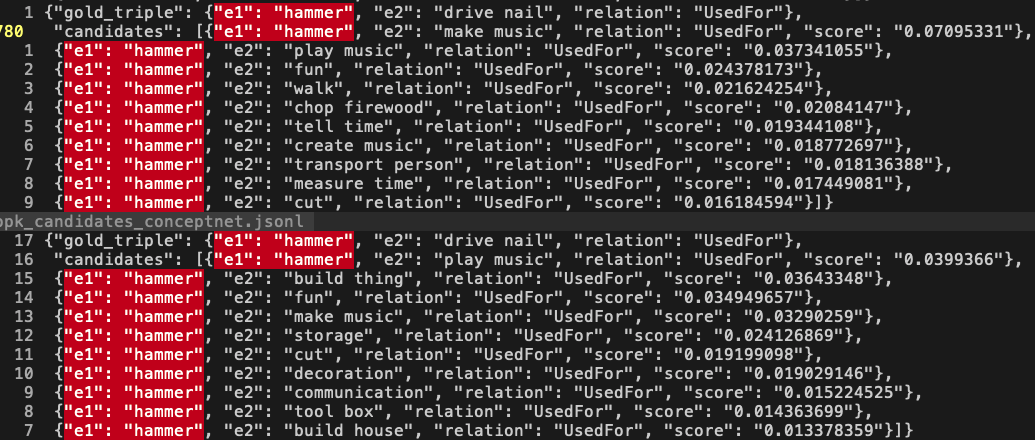
\includegraphics[scale=0.45]{images/hammer_top10_predictions.png}
    \caption{Hammer\_top10\_predictions. The top is from train ConceptNet alone and the bottom is from jointly training. Jointly train model is align before gcn embedding with pointwise pooling.}
    \label{fig:hammer-top10-prediction}
\end{figure}


The prediction files can be found at  \href{https://unimelbcloud-my.sharepoint.com/:f:/g/personal/chunhua_student_unimelb_edu_au/EuJ4GNdJNnFAmiDw7eE13oIBzBR7eJUrvyPRSEi8mrXIFw?e=bl9BcD}{here}
%\end{document}
